\documentclass[progress]{cmpreport}
\usepackage{natbib}
\usepackage{graphicx}
\usepackage{wrapfig}
\usepackage{paralist}
\usepackage{outlines}
\usepackage{booktabs}
\usepackage{appendix}
\usepackage{float}
\graphicspath{ {./} }

\title{Third Year Project: Progress Report}
\author{Matthew Taylor}
\registration{100151729}
\supervisor{Dr Rudy Lapeer}
\ccode{CMP-6013Y}

\begin{document}

\maketitle

\begin{section}{Introduction}

\subsection{Aim of the project}
The project aims to implement a first person video game which uses procedural generation (PCG) to provide a novel and interesting game experience. The project will explore the technical aspects of using PCG as a core feature of a game, specifically, implementation and performance. 

It will focus on real-time procedural level generation and providing a compelling, dynamic level structure.

\subsection{Motivation}
Procedural generation is not a new field, especially in video games, but there are interesting areas that are seldom explored.

The motivation behind the project's aims are to explore new and interesting concepts, namely, using PCG as a core feature in a game and using real-time procedural generation to provide an interesting experience.

\subsection{Literature}
The project also draws inspiration and guidance from existing PCG games, as described in papers by \citet{spufford_2003}, \cite{welsh_2016} and \cite{gct-spelunky}.

The project also takes into account the wealth of research done on PCG techniques, as described in papers by \cite{Perlin:1985:IS:325165.325247}, \cite{ebert2003texturing} and \cite{Dormans:2010:ALD:1814256.1814257}.
   
\end{section}

\begin{section}{Issues and problems}

This section will detail the issues identified at the project commencement and then detail how they have been addressed.

\subsection{Project scope}
Procedural content generation is a large field that has been explored in the literature since the 1980s. The paper by \cite{Hendrikx:2013:PCG:2422956.2422957} details this, providing a survey of PCG in games and the many techniques that have been used. A potential issue of the project is attempting to explore and implement too many of these techniques and ending up with a dilted project of little technical interest. 

To address this, the project scope was focussed on some areas identified as being under explored in the survey - level generation in real time systems. This will allow the project to explore several ideas in this domain and provide a comprehensive implementation in a fully featured game.

\subsection{Designing 3D games}
Designing 3D games and the assets required to populate the levels created could take a long time, especially if much of the functionality is created from scratch. 

To address this and enable the project to be achieved in a realistic timeframe, the Unity game engine was chosen. This tool enables relatively rapid production 3D game enviroments and assets, as well as being well documented and supported.

\subsection{Performance}
A game's performance is a critical aspect of its success. If the game cannot be played in a sustainable framerate on common hardware, it could be considered a techncial failure. Performance is a broad term, so the project will specifically focus on the following two aspects of performance. The first aspect is \textbf{level generation speed}. Each time the game loads, a new level is generated, so achieving a suitable speed in generating the levels and performing the associated work, like loading geometry, was a key consideration. The second aspect is \textbf{framerate}. The project will procedurally load a considerable amount of geometry in varied conditions. As much of the geometry will not be static, it will be required to load a large amount of meshes into memory, which could affect the performance.  

\subsection{Evaluation of success} \label{evalsuccess}
A key issue with this project is evaluating if it is successful. If there is no clear notion of what success looks like, the project could progress in unproductive directions. Below are the key measures of success chosen at the start of the project to measure success against.

\subsubsection{Convincing levels}
The levels must appear convincing. This is difficult to quantify, but nevertheless is an important attribute. The levels (at least in the initial design) will be mazes generated in a grid, with the grid sections subdivided in different ways.

This could easily create a boring level, where the grid pattern is discernable and the rooms are boring and procedural to traverse. Successful generation of levels will avoid these issues.

\subsubsection{Convincing decoration}
The decoration in each individual room will contribute to how convincing and hand-crafted each level looks. As described in \cite{doi:10.1111/j.1467-8659.2009.01351.x} and \cite{taylor-parberry}, there are several challenges to making room decoration appear to be hand-made when it is procedurally generated. Of particular focus will be generating furniture and objects in positions that feel realistic and unique.

\subsubsection{Performance}
Performance is another key component of the project succeeding. If the game responds poorly, it will be frustrating to play. Performance will be measured in a few ways:
\newline
\begin{compactitem}
    \item{\textbf{Framerate}: must be at least 30 frames per second}
    \item{\textbf{Initial loading time}: must take less than 30 seconds}
    \item{\textbf{Smooth level re-generation}: no dip in framerate below 30 frames per second}
\end{compactitem}



\end{section}

\begin{section}{Design and planning}

\subsection{Implementation methodology}
The project development operates under an Agile methology. Agile does not require that all requirements (or "user stories") are defined up front, instead it is encouraged that they are developed and refined during the lifecycle of the project.

The project itself is divided into Agile "sprints". It was decided to deliver a sprint every two weeks, as this fit with the development time given to the project and providing updates to the project supervisor.

While all the stories were not required at the outset, as part of the planning, it was decided to plot rough timescales against Agile "epics". These epics provide a high-level view of functionality and are detailed in Table \ref{tab:epics} in Appendix D.

The epics also contain very high-level user stories, which provide a little more detail. These were decided at the project outset, then refined during development. Before any user story can be developed, it is required that more detailed requirements are written. These are then recorded and tracked on Trello. 

\subsection{Implementation plan}

With the high-level design documented in the epics, planning of these epics against timescales was required. This timeline plan is visible in Figure \ref{fig:gantt1} in Appendix A. Progress was then tracked against this Gantt chart to ensure that progress was being made and that the project could be achieved as planned.

As the project is run using Agile principles, the Gantt chart has been revised to reflect changes to the plan. These changes are visible in Figure \ref{fig:gantt2} in Appendix A. Also included is the progress of the tasks so far.

Changes to the Gantt chart include the addition of a Level Generation task - the Level Re-Generator. This reflects a focus of the project on procedurally re-generating levels in real-time, so this has been split out as a seperate task and given a shorter timescale, reflecting the importance of the task to the project.

The gameplay section has been split into two tasks, reflecting the focus on implementing core gameplay as a priority, with enhanced gameplay being desirable but not as critical to the evaluation of success of the project.


\subsection{UML}

As the project began, a UML diagram was designed to provide a high level framework to work towards. Unity does not prescribe much structure, so a UML design to begin with was useful. The initial UML design can be seen in Figure \ref{fig:uml1} in Appendix B. The iterated design can be seen in Figure \ref{fig:uml2} in Appendix B, which shows the definition of classes being enhanced with the additional methods and attributes required to support the design, as well as the addition of the \textbf{Level Re-Generator} class.


\subsection{Requirements and prioritisation}

The project defined epics (or, high level requirements) at the outset, with more detailed requirements written at each stage. This allows the project the be flexible, with lessons learned in the prototyping incorporated into future requirements. It also saves time, because requirements do not need to be written in advance when they would likely be changed anyway.

The epics and requirements written for the project so far are available in the appendix in Table \ref{tab:epicreqs} on \pageref{tab:epicreqs}.


\subsection{Design prototypes}
\subsubsection{Guaranteed path generation}
The first part of the design to be implemented required a guaranteed path through a maze to be generated. This was achieved by using a random walk - a stochastic process implmented in two dimensions to provide a definite route through the maze.

The random walk is implemented using an agent based approach. The agent can choose from three random directions to travel in - left, right or down. These probabilities are detailed in Table \ref{tab:probdirs}. When the agent has chosen a valid direction, it randomly selects a valid tile. 

The agent has methods of checking where it has been and where it is going next, so that it picks valid tiles that have openings in the directions it has come from and intends to go. The agent is given bounds and restrictions while it is performing the random walk, which provides a method of parameterising the level and deciding on an endpoint. 

\subsubsection{Decoration of rooms}

Rooms are decorated with interior sub-dividing walls and other elements to provide a convincing and interesting environment to traverse. Decoration is achieved by populating each room with a random pre-defined set of geometry, examples of which can be seen in Figures \ref{fig:prefab-room}, \ref{fig:prefab-int} and \ref{fig:room}, in Appendix C. 

In the prototype design, a single point is used to populate all geometry from the centre of the room. However, iterations on the design will use several points which an agent will scan through to populate things like sub-rooms, corridors, walls and desks with appropriate decorations, providing considerable variation for little asset generation cost.

\end{section}

\begin{section}{Evaluation of progress}

\subsection{Progress against plan}
As detailed in the revised Gantt chart in Figure \ref{fig:gantt2} in Appendix A, progress is broadly on plan. The prototyping of the level and room generation is complete and suitable methods have been implemented. Much of the remaining work on level and room generation will focus on refining the performance, achieving higher levels of complexity and improving performance.

\subsection{Changes to plan}
The plan has changed slightly since the project began. As can be seen in the differences between Figure \ref{fig:gantt1} and Figure \ref{fig:gantt2} in Appendix A, two new tasks have been added.

The \textbf{Level Re-generator} task has been added and given a shorter timeframe to provide focus on this task. The re-generation aspect of the project is important to consider when evaluating performance It also provides a novel feature not seen in many computer games, so this was considered important to focus on.

The \textbf{Add Enhanced Gameplay} task was also added, to provide a marked difference between the basic implementation and a more detailed gameplay experience. It will not require much effort to provide a basic experience, which will be important to implement early. The project will then consider enhanced gameplay elements (more enemies, pickups, keys for locked doors) towards the end of the project, after the main aims have been achieved.

\subsection{Evaluation against success measures}
In Section \ref{evalsuccess} on page \pageref{evalsuccess}, three measures of success for the project were defined. 

Against the \textbf{Convincing Levels} measure, the project has the potential to succeed. The guaranteed path/tile filling combination creates large levels, with a path through them. The project does not currently take steps to block off many of the non-guaranteed path tile transitions, so the tile structure is discernable - it is quite easy in parts to see how the tiles are laid out. Future 

Against the \textbf{Convincing Decoration} measure, the project again has the potential to succeed. The prototype of the room decoration system works, but would require quite a lot of manual content generation. However, the project has also successfully implemented agent based approaches to creating levels, so a combination of hand-crafted content and procedural generation should enable rooms to be decorated in ways that are procedural and unique, but also in ways that make sense to humans.

Against the \textbf{Performance} measure is where the project has faced the most challenges. The level generation algorithm is quite efficient. As presented in Figure \ref{tab:gentimes} in Appendix D, even when large sizes are used the generation and instantiation time does not increase by much. Indeed, the main constraint around generating large levels is not the time to generate them, but the real-time performance of the levels.

The real-time aspect suffered when large levels were generated. Average framerate was low (around 10 FPS) when levels and decoration was applied to suitable level sizes for a playable game. This resulted from a lack of occlusion culling and a large draw distance. This was overcome by reducing the viewing frustrum size from it's default size to one more suitable for navigating a closed maze-like level, as demonstrated in Figure \ref{fig:frustrums} on page \ref{fig:frustrums}. Global shadow quality was also reduced. These changes resulted in a change of the average framerate from 10 FPS to 60 FPS - well above the threshold required by the performance metric.

\end{section}

\begin{section}{Conclusion}
To conclude, the project is progressing well against the plan. The project is also meeting the success measures decided at the start of the project.

The project has so far just implemented prototype systems, but the systems are extensible and scalable. The framework implemented will easily allow gameplay elements to be added and for increased graphical fidelity to be achieved. 

This provides a high level of confidence that the project can achieve the objectives of being interesting, fun and of high graphical quality.

\end{section}

\bibliography{sources}

\newpage

\appendix

\begin{section}{Gantt charts}

\begin{figure}[H]
    \centering
    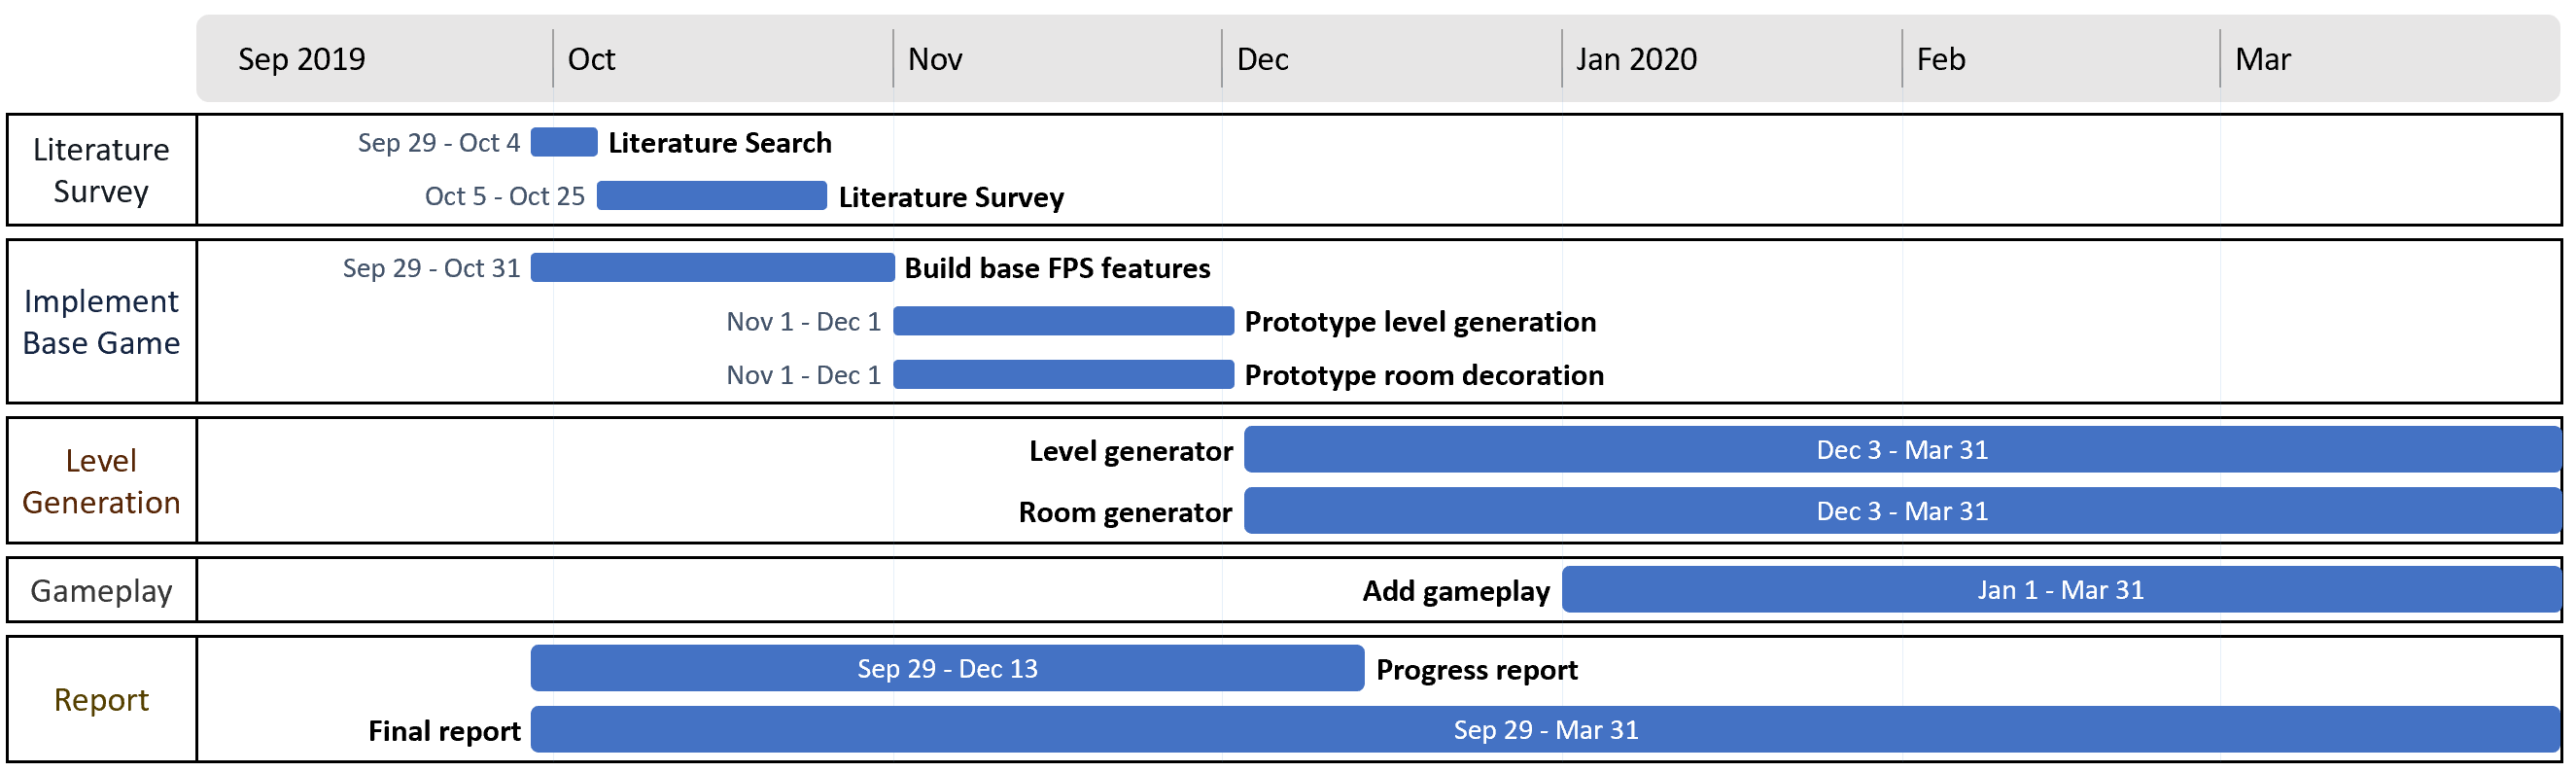
\includegraphics[angle=90,width=\textwidth,height=0.85\textheight,keepaspectratio]{img/gantt-original2.png}
    \caption{Gantt chart of original plan}
    \label{fig:gantt1}
\end{figure}

\begin{figure}[H]
    \centering
    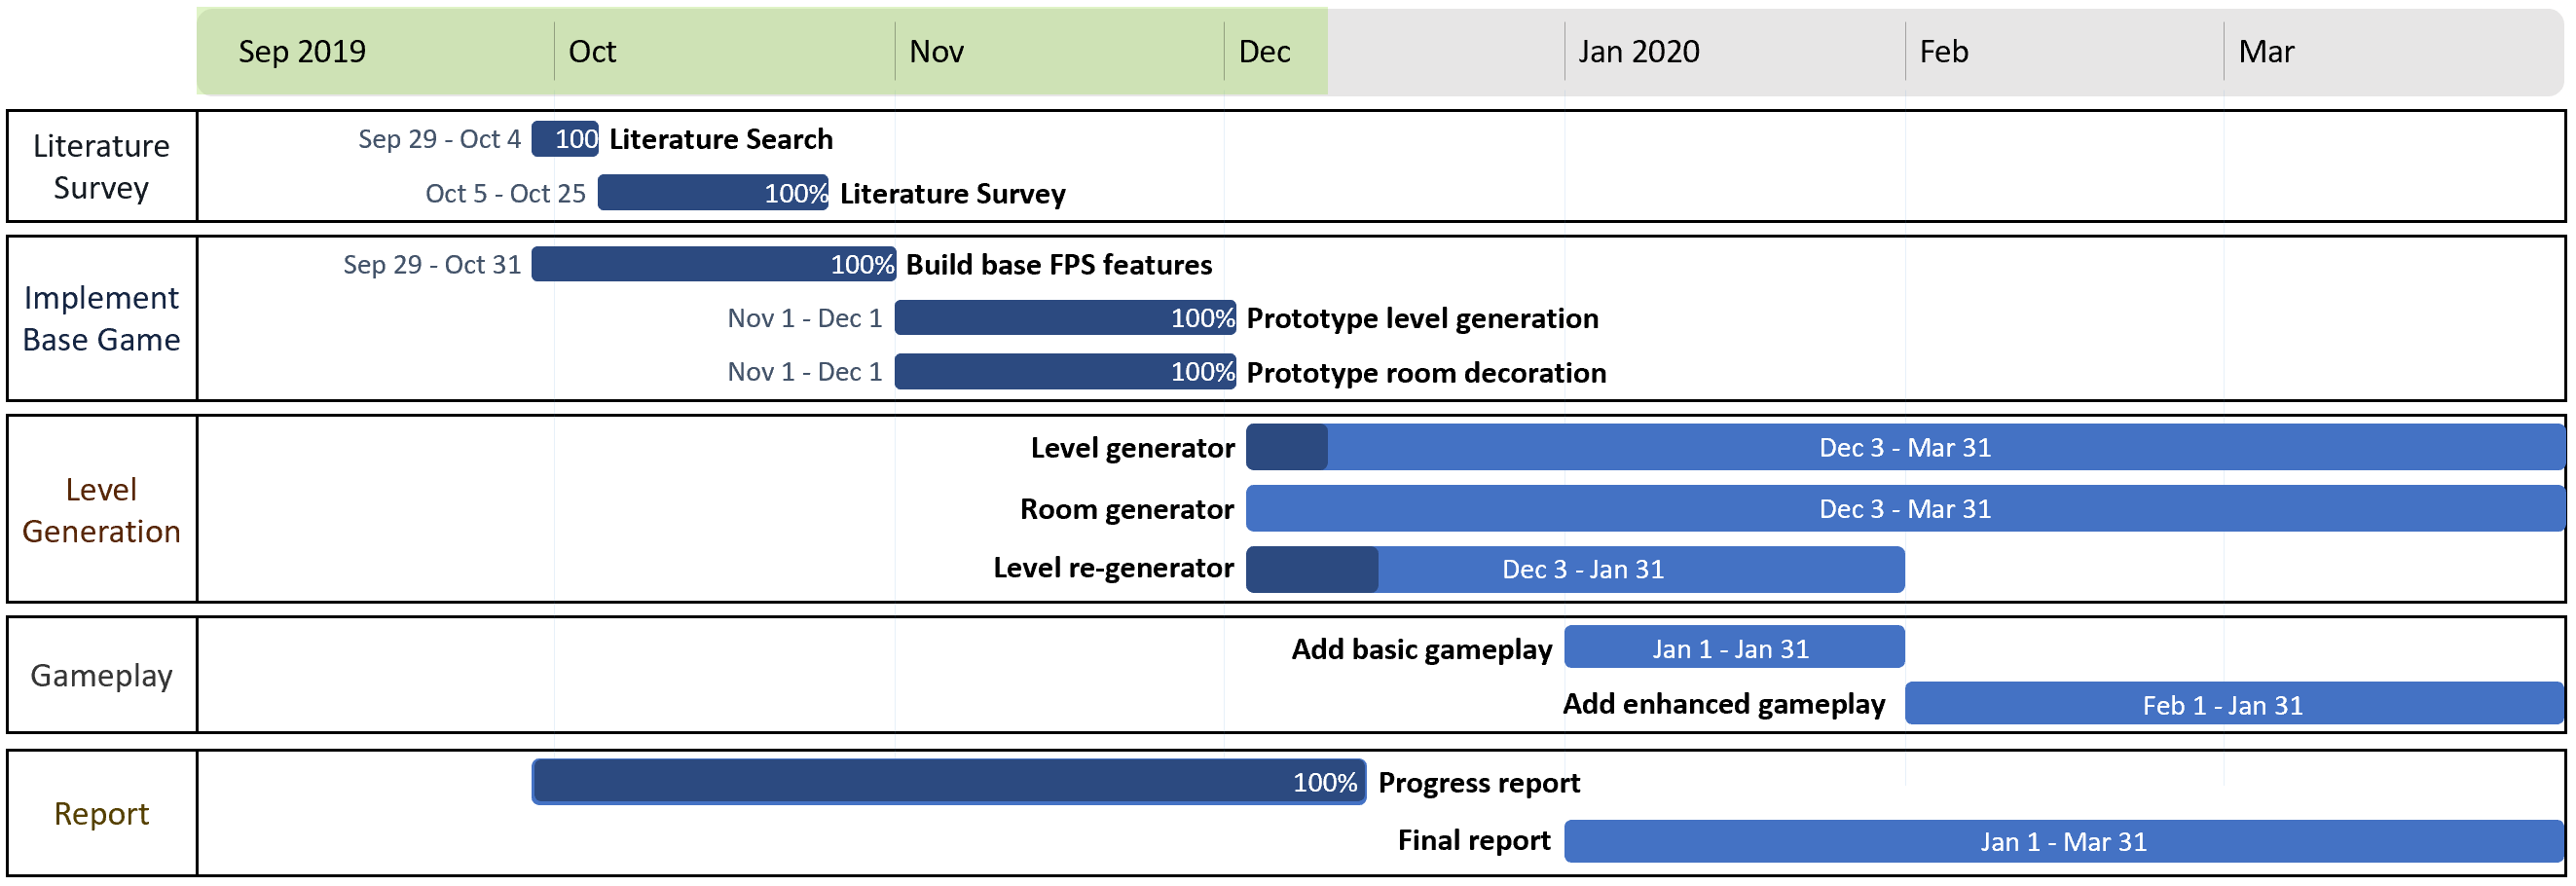
\includegraphics[angle=90,width=\textwidth,height=0.85\textheight,keepaspectratio]{img/gantt-updated2.png}
    \caption{Gantt chart of updated plan}
    \label{fig:gantt2}
\end{figure}

\end{section}

\begin{section}{Diagrams}

\begin{figure}[H]
    \centering
    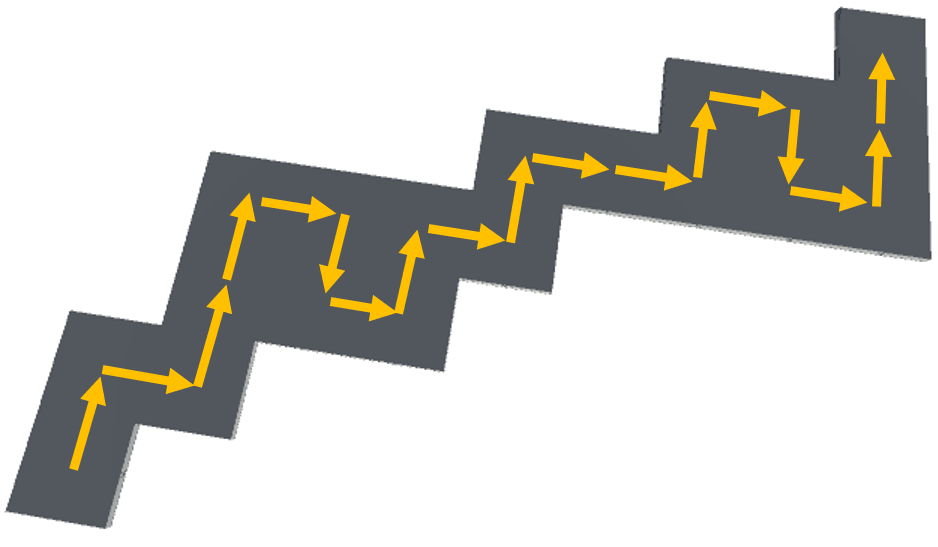
\includegraphics[width=8cm]{img/1-maze.png}
    \caption{A top-down view of the guaranteed path generation, showing how the PCG algorithm moves in three directions to create a route through a maze}
    \label{fig:pathgen}
\end{figure}

\begin{figure}[H]
    \centering
    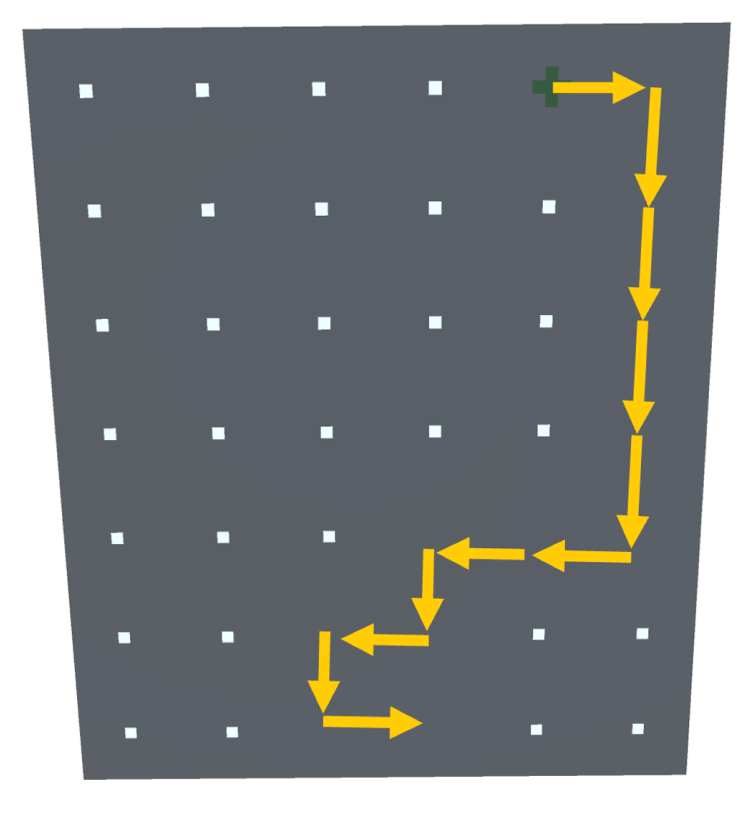
\includegraphics[width=8cm]{img/filled-path.png}
    \caption{A top-down view of the guaranteed path with remaining tiles filled in, demonstrating how the filling algorithm works}
    \label{fig:filledpath}
\end{figure}

\begin{figure}[H]
    \centering
    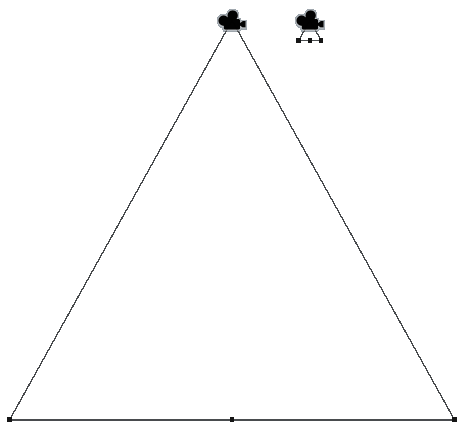
\includegraphics[width=8cm]{img/frustrums.png}
    \caption{A top-down of the difference in default and optimised viewing frustrum sizes, with Unity's default frustrum size on the left and the optimised size for the generated mazes on the right}
    \label{fig:frustrums}
\end{figure}

\begin{figure}[H]
    \centering
    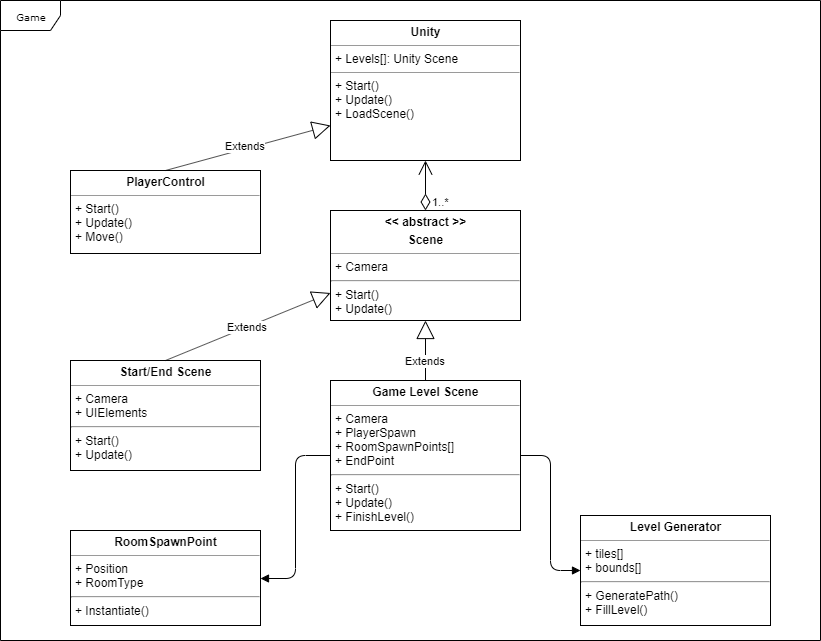
\includegraphics[width=\textwidth]{img/uml1.png}
    \caption{Initial UML diagram}
    \label{fig:uml1}
\end{figure}

\begin{figure}[H]
    \centering
    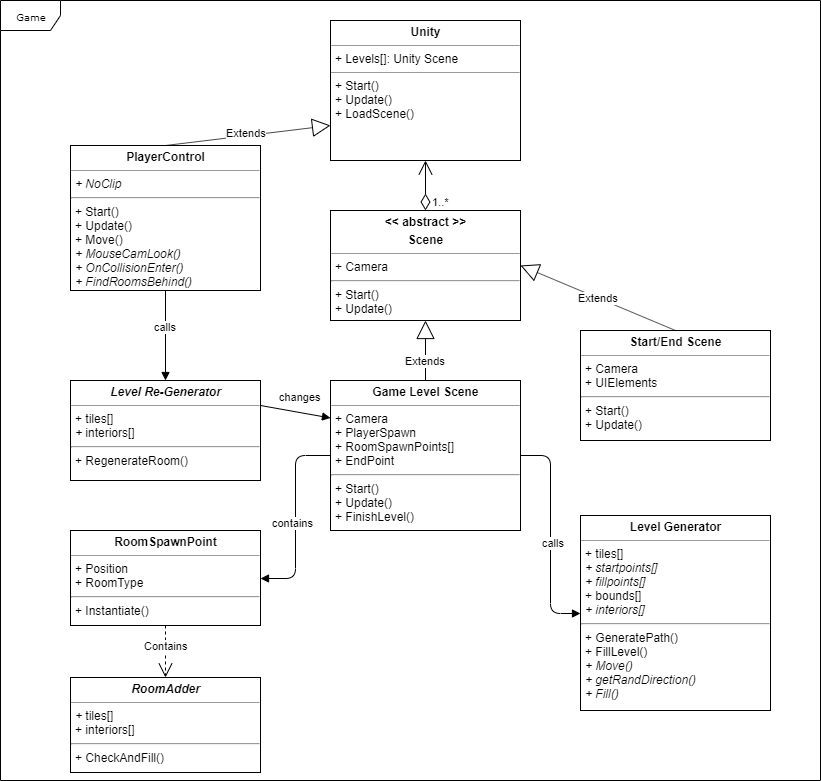
\includegraphics[width=\textwidth]{img/uml2.png}
    \caption{Redesigned UML diagram}
    \label{fig:uml2}
\end{figure}



\end{section}

\begin{section}{Screenshots}
    


\begin{figure}[H]
    \centering
    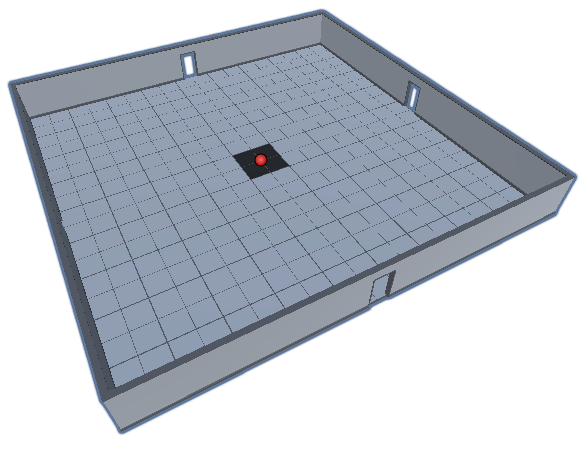
\includegraphics[width=.8\textwidth]{img/prefabroom.png}
    \caption{A screenshot of a room tile, showing the walls and exits of a tile (with the ceiling hidden)}
    \label{fig:prefab-room}
\end{figure}

\begin{figure}[H]
    \centering
    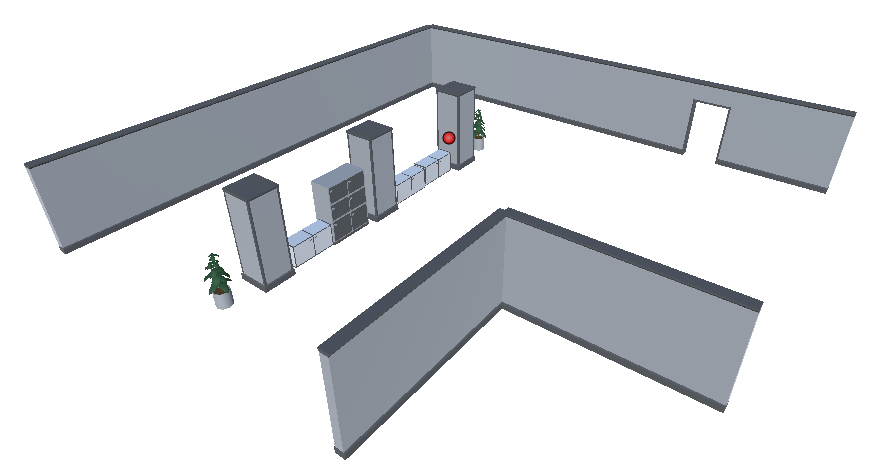
\includegraphics[width=.8\textwidth]{img/interior.png}
    \caption{A screenshot of a room interior, designed to fit into any tile with any exit}
    \label{fig:prefab-int}
\end{figure}

\begin{figure}[H]
    \centering
    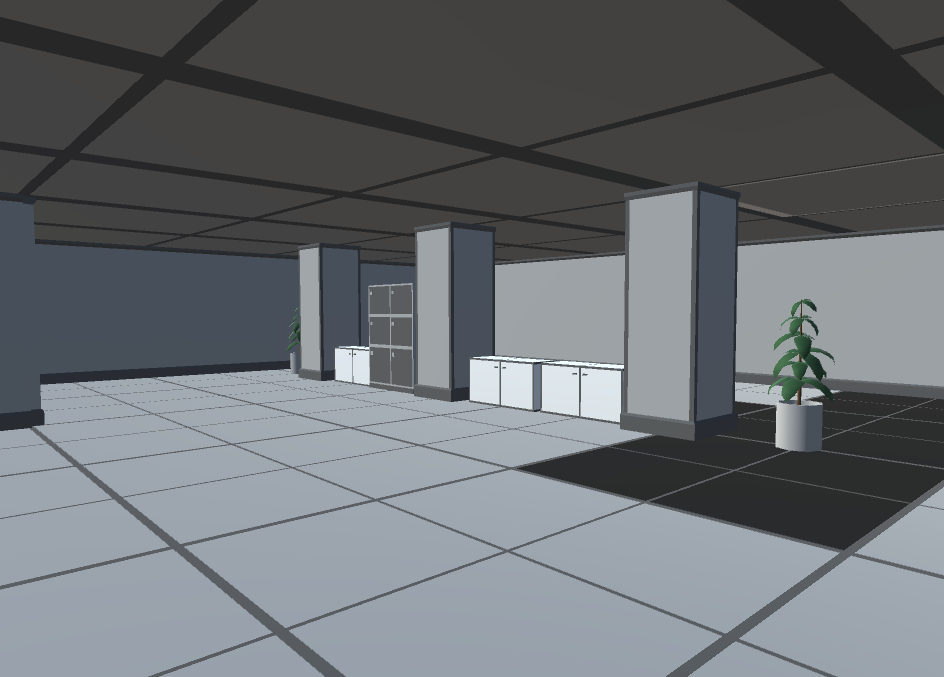
\includegraphics[width=.8\textwidth]{img/imp-int.png}
    \caption{A screenshot of a procedurally generated room, with the tile and interior composited in a real-time environment}
    \label{fig:room}
\end{figure}



\end{section}

\newpage
\begin{section}{Tables}

% epic/story table
\begin{table}[H]
    \resizebox{\textwidth}{!}{%
    \begin{tabular}{@{}ll@{}}
    \toprule
    \multicolumn{1}{l|}{\textbf{Epic}} & \textbf{Stories} \\ \midrule
    \multicolumn{2}{l}{Build base "first person" 3D game features} \\
     & Provides a basic level design \\
     & Proves the concepts of vision and movement \\ \midrule
    \multicolumn{2}{l}{Prototype level generation} \\
     & Prove a method of generating a guaranteed path through a maze \\
     & Prove a method of filling in non-guaranteed paths through the maze \\ \midrule
    \multicolumn{2}{l}{Prototype room generation} \\
     & Prove a method of generating room interiors \\
     & Room generation must not interfere with guaranteed path \\ \midrule
    \multicolumn{2}{l}{Prototype level re-generation} \\
     & Design method to procedurally re-generate level sections \\ \midrule
    \multicolumn{2}{l}{Add gameplay elements} \\
     & Decide on how level is finished by the player \\
     & Provide some interest and threat when playing \\
     & Provide means of assisting navigation \\ \midrule
    \multicolumn{2}{l}{Implement final designs} \\
     & Use non-prototype textures \\
     & Ensure performance meets goals \\ \bottomrule
    \end{tabular}%
    }
    \caption{Agile-style epics and associated user stories}
    \label{tab:epics}
\end{table}

% Please add the following required packages to your document preamble:
% \usepackage{graphicx}
\begin{table}[H]
    \resizebox{\textwidth}{!}{%
    \begin{tabular}{llll}
    \hline
    \multicolumn{1}{|l|}{\textbf{Requirement type}} & \multicolumn{1}{l|}{\textbf{Requirement}} & \multicolumn{1}{l|}{\textbf{Priority}} & \multicolumn{1}{l|}{\textbf{Status}} \\ \hline
    Epic & Write Project Proposal & Should Have & Done \\
    - Requirement & Research PCG & Should Have & Done \\
    - Requirement & Write proposal & Should Have & Done \\ \hline
    Epic & Write Literature Review & Should Have & Done \\
    - Requirement & Research/find literature & Should Have & Done \\
    - Requirement & Get feedback & Should Have & Done \\
    - Requirement & Write review & Should Have & Done \\ \hline
    Epic & Build base FPS features & Must Have & Done \\
    - Requirement & Create title/game over screens & Should Have & Done \\
    - Requirement & Create end goal, transitions to end screens & Should Have & Done \\
    - Requirement & Implement first person controller & Must Have & Done \\ \hline
    Epic & Prototype level generation & Must Have & Done \\
    - Requirement & Design room tile prefabs & Must Have & Done \\
    - Requirement & Implement "random walk" generation & Must Have & Done \\
    - Requirement & Implement maze filling algorithm & Must Have & Done \\
    - Requirement & Implement different sized tiles & Could Have &  \\ \hline
    Epic & Prototype room decoration & Must Have & Done \\
    - Requirement & Design room decoration prefabs & Must Have & Done \\
    - Requirement & Implement room decoration filling algorithm & Must Have & Done \\
    - Requirement & Design random sub-decorator agents & Could Have & Done \\ \hline
    Epic & Progress report & Must Have & Done \\
    - Requirement & Design plan & Should Have & Done \\
    - Requirement & Write first draft & Should Have & Done \\
    - Requirement & Write final draft and submit & Must Have &  \\ \hline
    Epic & Prototype re-generation & Must Have &  \\
    - Requirement & Design approach for re-generating parts of level in real-time & Must Have &  \\
    - Requirement & Implement re-generation process & Must Have &  \\
    - Requirement & Implement re-generation trigger process & Must Have &  \\ \hline
    Epic & Level generator & Must Have &  \\ \hline
    Epic & Room generator & Must Have &  \\ \hline
    Epic & Level re-generator & Must Have &  \\ \hline
    Epic & Basic gameplay & Must Have &  \\ \hline
    Epic & Enhanced gameplay & Should Have &  \\ \hline
    Epic & Final report & Must Have &  \\ \hline
    \end{tabular}%
    }
    \caption{A table showing epics and requirements, their priorities and statuses}
    \label{tab:epicreqs}
\end{table}

\begin{table}[h!]
    \centering
    \begin{tabular}{ |c|c|c| }
    \hline
    \textbf{Left} & \textbf{Right} & \textbf{Down} \\ 
    \hline
    40\% & 40\% & 20\%\\ 
    \hline
    \end{tabular}
    \caption{A table showing probability of direction random walk agent will take}
    \label{tab:probdirs}
\end{table}

\begin{table}[]
    \centering
    \begin{tabular}{|l|l|}
    \hline
    \textbf{Level size} & \textbf{Generation time} \\ \hline
    4 x 6 & 6.34 seconds \\ \hline
    6 x 10 & 6.89 seconds \\ \hline
    15 x 30 & 7.28 seconds \\ \hline
    30 x 50 & 9.61 seconds \\ \hline
    70 x 100 & 13.20 seconds \\ \hline
    \end{tabular}
    \caption{A table showing the project's level sizes in tiles and time it takes the procedural algorithms to generate the levels}
    \label{tab:gentimes}
    \end{table}

\end{section}

\end{document}
